%% ------------------------------------------------------------------------- %%
\chapter{Introdução}
\label{cap:introducao}


A durabilidade e vida útil do cimento tem sido o problema mais importante enfrentado pela indústria de construção civil nas últimas décadas \citep{cementml}. Os custos de manutenção são da ordem de bilhões de dólares e portanto, a capacidade da previsão de propriedades do cimento desde a sua produção ganha grande importância. Une-se a isso a presença cada vez maior de métodos de ML em domínios diversos da engenharia e ciência com excelentes resultados e surge então a tentativa de usar algoritmos de aprendizado também para esse domínio \citep{cementnn1, cementnn2}. \\ 

Esse trabalho é uma colaboração entre a empresa Intercement e o Laboratório de
Lógica, Inteligência Artificial e Métodos Formais do IME-USP. Foram concedidos
10 anos de dados de diversas etapas da produção de cimento do complexo de
Cajati, uma das plantas da empresa. Esse trabalho é um estudo com a análise
desses dados, desde o seu pré-processamento até uma criação de modelos
preditivos e a investigação de sua acurácia. \\

O indicador mais usado para a qualidade do cimento é a Resistência Compressiva (CSC) discutida na Sessão~\ref{sec:rc}, medida em quilo-pascais (kPa). Normas exigem que a CSC da amostra 28 dias após a sua expedição pela fábrica
cumpra certos requisitos. Esse valor, o RC28, é o principal objetivo de predição de modelos estatísticos propostos na literura, visto que é de grande valia uma estimativa confiável desse valor antes que o mesmo seja medido por análise laboratorial 28 dias após a produção da amostra em questão. Concentrações de reagentes e outras grandezas referentes ao processo industrial são então usados em uma tarefa de \textbf{aprendizado supervisionado} para predizer o valor do RC28. \\


\section {Motivação}


Muito da literatura proposta para esse problema falha em levar em consideração o processo industrial da produção de cimento, e se limitam a análise de dados estritamente no contexto laboratorial \citep{cementlin},\citep{nncement}, com análises que não poderiam ser feitas no dia-a-dia da fábrica \citep{dynstat}. \\

Mas trabalhos recentes propõe métodos de modelagem que poderiam ser implementados em chão de fábrica. \cite{greciaLin,dynstat} usam uma regressão linear de janela móvel, recalculando parâmetros de regressão sempre que uma nova medida RC28 é entregue pelo laboratório. Os dados então passam a ser tratados temporalmente, a medida que eles se tornam disponíveis na fábrica. Esse trabalho irá continuar nesse caminho e irá considerar os dados fornecidos da produção de cimento como \textbf{séries temporais}, assumindo que existe uma correlação entre lotes de cimento temporalmente próximos na expedição da fábrica. Nosso objetivo será o de modelar a \textbf{distribuição de probabilidade} dessa série, de modo a podermos amostrar médias e variâncias úteis para análise diária na fábrica. 

Por muitas décadas o estado da arte desse tipo de análise temporal foram os processos ARIMA, com a metodologia Box-Jenkins \citep{arima}. Esses modelos tem uma excelente capacidade estatística e interpretabilidade. Mas essa família de modelos não vem sem as suas limitações: Eles falham em modelar relações não-lineares nos dados \citep{forecasting}, e a muitos processos reais tendem a ser não-lineares por natureza.

Novos métodos de Machine Learning (ML) e mais recentemente Deep Learning (DL) como Redes Neurais Profundas (DNN), tem conquistado melhores resultados em diversas campos como visão computacional, análise de linguagem narutal (NLP) e regressão de séries temporais. Modelos de DL diferem de abordagens estatísticas clássicas por serem orientados a dados \citep{dlbook}. Esses modelos não necessitam de \textit{feature engineering}, e também não assumem muito sobre a distribuição geradora dos dados, como por exemplo a família ARIMA, que requisita do engenheiro de dados a especificação da sazonalidade e estacionariedade dos dados \citep{arima}. Redes Neurais são capazes de aprendem sozinhas diversas caractísticas dos dados sem necessidade de intervenção. \\

Alguns trabalhos uniram a flexibilidade de DNNs com a robustez de métodos ARIMA \citep{DIAZROBLES20088331,KHASHEI2010479}, criando soluções melhores que qualquer um desses modelos sozinho.
Outro modelo de DL que obteve excelentes resultados empíricos foram Redes Neurais Recorrentes, modelos sequenciais usados para NLP e também análise de séries temporais. Esses modelos já foram usados com resultados melhores que o estado da arte para prever séries temporais de demanda de energia elétrica e de carros em um aplicativo de corridas popular \cite{energylstm,ubertime}. Uma tendência recente agora é de usar modelos de Deep Learning Bayesianos, que unem a versatilidade de modelos de DL com a expressividade de técnicas bayesianas, capazes de modelar a distribuição de probabilidade alvo pela Lei de Bayes. Esse trabalho irá aplicar 3 técnicas recentes de regressão de séries temporais com métodos bayesianos na predição do CSC do cimento. São elas:




%% ------------------------------------------------------------------------- %%
\section{Produção de Cimento}
\label{sec:producao}

Nessa seção será feito um breve resumo da produção de cimento, usando como base na Figura~\ref{fig:cement}: \\ 

\begin{figure}[H]
\label{fig:cement}
\centering
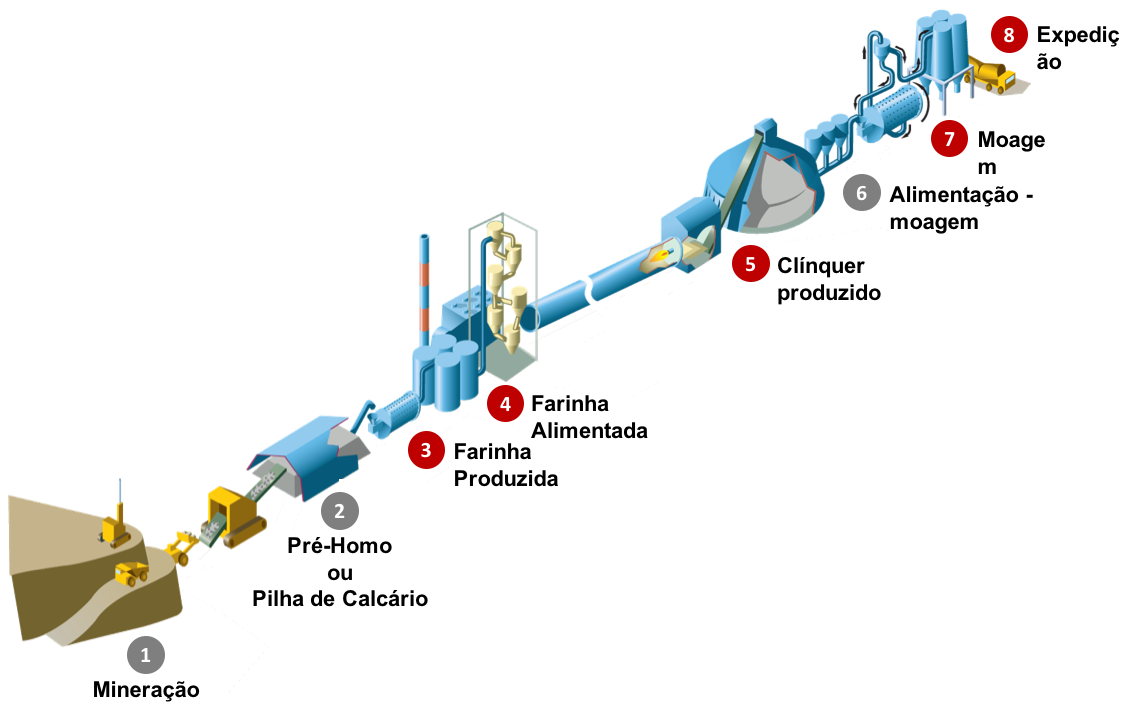
\includegraphics[width=0.9\columnwidth]{cimento.png}
\caption{Representação das Diversas Etapas da produção de Cimento \citep{cementroadmap}}
\end{figure}


As etapas de produção serão explicadas por número como indicado na imagem: \\

\begin{itemize}

\item[1] Depósitos ricos em carbonato de cálcio são mineirados para extração desse químico. Normalmente a planta é próxima da mina.
\item[2] O material extraido é triturado em pedaços de até 10cm. Diferentes materiais são misturados ao resultado da tritura, de modo a manter a composição química desejada. 
\item[3] A farinha crua é pré-aquecida para que depois no forno as reações químicas aconteçam mais rápido. 
\item[4] O cálcio é transformado em CaO por meio de reações químicas.  
\item[5] O material é introduzido ao forno, atingindo temperaturas de até $1450^\circ$C, transformando a farinha em clínquer. O clínquer é resfriado após a saída do forno. 
\item[6] O clínquer então é misturado com outros componentes que formam o cimento.
\item[7] A mistura é então moída.
\item[8] O material é empacotado, estocado e eventualmente expedido para entrega.

\end{itemize}

Os dados são medições de diversos parâmetros em meio ao processo de fabricação do cimento. Eles são divididos em diversas planilhas para diferentes etapas da produção de cimento, são elas, em ordem no processo:

\begin{itemize}
        \item Cimento Cru
        \item Farinha
        \item Clinquér
        \item Produção de Cimento
        \item Expedição de Cimento (Saco e Granel)
\end{itemize}

Dado que não existe uma maneira trivial de combinar dados de partes diferentes do processo (é muito difícil acompanhar o mesmo lote de cimento/matéria prima em partes diferentes do processo), as análises serão feitas em cima dos dados de Expedição de Cimento.

\subsection{Índice de Resistência de Cimento Portland}
\label{sec:rc}
A propriedade que iremos tentar prever usando nossos modelos será a resistência
compressiva do cimento. A resistência de uma amostra de cimento é ensaiada em
intervalos determinados de dias após a sua confecção. Essas informações são
anotadas nos dados com os nomes de $RCX$, com $X$ sendo a idade da amostra em
dias. Esses índices possuem a únidade de kPa, i.e. quilopascal.

%% ------------------------------------------------------------------------- %%
\section{Objetivos}
\label{sec:objetivo}

Gostariamos no desenvolvimento desse trabalho de obter resultados com a
aplicação de técnicas de DL recentes para um domínio inédito. Dessa maneira
abrindo portas para uma presença de aprendizado estatístico no processo de
engenharia da produção de cimento. De modo que esses modelos possam ser usados para tomadas de decisão no chão de fábrica.


%% ------------------------------------------------------------------------- %%
\section{Organização do Trabalho}
\label{sec:organizacao_trabalho}

No Capítulo~\ref{cap:conceitos}, apresentamos os conceitos de Aprendizado de
Máquina, estatística frequentista e bayesiana, além de uma breve explicação
de cada modelo usado. No Capítulo~\ref{cap:estudodados} é mostrado de que
maneiras os dados foram tradados e modificados para facilidade de sua modelagem.
No Capítulo~\ref{cap:resultados} constam os resultados dos ensaios feitos com os dados. 



%%% Local Variables:
%%% mode: latex
%%% TeX-master: "../quali"
%%% End: